\section{Back-end}

\subsection{Back-end}
\begin{frame}
    \frametitle{Back-end}
    The backend is responsible for creating an executable
\end{frame}

\begin{frame}
    \frametitle{Goals}
    \begin{enumerate}
    \item generate executable code from the typechecked AST
    \item verify the correctness of the generated code 
    \item embed an interactive debugger in the executable
    \end{enumerate}
\end{frame}

\begin{frame}
    \frametitle{\subsecname}
    \framesubtitle{Requirements}
    Hard requirements
    \begin{itemize}
    \item Must inter-operate with .Net
    \item Must be multi-platform
    \item Must generate correct code
    \end{itemize}
    Soft requirements
    \begin{itemize}
    \item Faster is better
    \end{itemize}
\end{frame}

\begin{frame}
    \frametitle{\subsecname}
    \framesubtitle{Native solutions}

    \begin{itemize}
        \item Can use the fast LLVM C/C++ code generator
        \item Requires hand-written garbage collector
        \item May not have privileges on mobile platforms
    \end{itemize}

    \begin{tabular}{l|l|l}
        & multi-platform & speed \\
        \hline
        P/Invoke      & not on mobile & control flow with .Net\\
        wrapper DLL   & windows only  & very high overhead \\
        hosted        & windows only  & no high-speed JIT \\
    \end{tabular}

    \begin{itemize}
        \item None good enough
    \end{itemize}
\end{frame}

\begin{frame}
    \frametitle{\subsecname}
    \framesubtitle{Managed solutions}

    \begin{itemize}
        \item High reliability, no hybrid constructs
        \item Uses the fast .Net garbage collector
    \end{itemize}

    \begin{tabular}{l|l|l|l}
        & multi-platform & speed & other\\
        \hline
        C++/CLI & on windows & fast & horrible in every way\\
        F\#     & everywhere & slow & resists imperative code\\
        CIL     & everywhere & fast & difficult to debug\\
        C\#     & everywhere & fast & Most supported compiler\\
    \end{tabular}

    \begin{itemize}
        \item C\# is the best choice
    \end{itemize}
\end{frame}

\begin{frame}
    \frametitle{\subsecname}
    \framesubtitle{The AST}
    \begin{itemize}
    \item The interface between the front-end and the back-end
    \item Contains
        \begin{itemize}
        \item All the functions
        \item All the data declarations
        \item The “main” function
        \item The compiler flags
        \end{itemize}
    \item All types are already inferenced and typechecked
    \item All generics are already reified/concrete
    \end{itemize}
\end{frame}


\subsection{Code Generation}

\begin{frame}[fragile]
    \frametitle{\subsecname}
    \framesubtitle{Normalization}
    \begin{multicols}{2}
    \begin{lstlisting}


-------------
count [] -> 0







count xs -> res
--------------------
count x::xs -> res+1
    \end{lstlisting}
    \columnbreak
    \begin{lstlisting}
_tmp0 -> []
0 -> _tmp1
--------------------
count _tmp0 -> _tmp1

_tmp0 -> x::xs
count -> _tmp1
_tmp1 xs -> res
(+) -> _tmp2
_tmp2 res -> _tmp3
1 -> _tmp4
_tmp3 _tmp4 -> _tmp5
--------------------
count _tmp0 -> _tmp5
    \end{lstlisting}
\end{multicols}
\end{frame}

\begin{frame}[fragile]
    \frametitle{\subsecname}
    \framesubtitle{Rule structure}
    \begin{lstlisting}
    \end{lstlisting}
\end{frame}

\begin{frame}[fragile]
    \frametitle{\subsecname}
    \framesubtitle{Func structure}
    \begin{lstlisting}
Class MyFunc {
    <function arguments>
    public <return type> run() {
        {
            <rule 1 implementation>
            return <local>;
        }
      skip1:
        {
            <rule 2 implementation>
            return <local>;
        }
      skip2:
        throw exception
    }
};
    \end{lstlisting}
\end{frame}

\begin{frame}[fragile]
    \frametitle{\subsecname}
    \framesubtitle{Data structure generation}
    \begin{lstlisting}
Data "Left"  -> string -> string | float
Data "Right" -> float  -> string | float
    \end{lstlisting}
    
    \begin{lstlisting}
Class _pipe {};
Class _Left :_pipe {string _arg0;};
Class _Right:_pipe {float  _arg0;};
    \end{lstlisting}
\end{frame}

\begin{frame}[fragile]
    \frametitle{\subsecname}
    \framesubtitle{Mangler}
    \begin{itemize}
        \item Transforms valid Mc identifiers to valid C\# identifiers
        \item The escape character is underscore
        \item \verb/!/ becomes \verb/_bang/, \verb/|/ becomes \verb/_pipe/, \verb/_/ becomes \verb/_under/
        \item C\# keywords are prefixed with @. @if, @int, etc.
        \item Non-ascii symbols are converted to utf-8 NFD.\\
              $\vcenter{\hbox{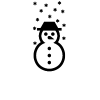
\includegraphics[height=1.5em]{snowman}}}$ becomes \verb/_E2_98_83/
        \item Type information is also suffixed with \verb/_T/, \verb/_L/ and \verb/_R/.\\
            (list(list int)) becomes \verb/_Llist_Llist_Tint_R_R/
    \end{itemize}

\end{frame}
\subsection{Verification}
\begin{frame}
    \frametitle{\subsecname}
    \framesubtitle{interpreter}
\end{frame}

\subsection{Debugger}

\begin{frame}
    \frametitle{\subsecname}
    \framesubtitle{GUI}
    \begin{figure}
        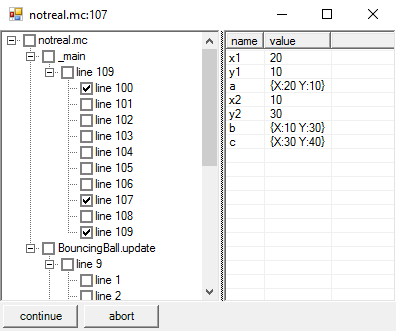
\includegraphics[scale=0.5]{debugger}
    \end{figure}
\end{frame}

\begin{frame}
    \frametitle{\subsecname}
    \framesubtitle{program tree}
\end{frame}

\begin{frame}
    \frametitle{\subsecname}
    \framesubtitle{break points}
\end{frame}

\begin{frame}
    \frametitle{\subsecname}
    \framesubtitle{Local definitions}
\end{frame}

